% =============================================================================
% Section 6 — Mutation Accumulation
% =============================================================================
\section{Mutation Accumulation: Reading Rates from Fluctuations}\label{sec:accumulation}

\begin{objectives}
\begin{itemize}[leftmargin=*,itemsep=1pt,topsep=1pt]
  \item Explain why the \emph{mean} number of mutants is a poor estimator of a mutation rate.
  \item Derive the overdispersion that distinguishes pre-existing mutation from induced adaptation.
  \item Simulate the Luria--Delbrück process and recover its signature numerically.
  \item Connect the fluctuation test to the rate measurements used in Section~\ref{sec:refutation}.
\end{itemize}
\end{objectives}

\subsection{Biological setting}

Section~\ref{sec:refutation} quoted mutation rates: $44 \times 10^{-8}$ for
\texttt{pol2-4}, $2300 \times 10^{-8}$ for \texttt{pol2-P301R}. Those numbers did
not come from counting mutants and dividing. They came from a fluctuation
analysis, and understanding why is essential to trusting them.

The problem is that mutations arise \emph{during} growth. A mutation in the first
division is inherited by half the final population; one in the last division
yields a single mutant cell. Two cultures with identical mutation rates can
therefore end with wildly different mutant counts, and the distribution of those
counts is not Poisson.

\subsection{Mathematical development}

\begin{model}[Luria--Delbrück process]\label{model:ld}
A culture starts from one wild-type cell and grows for $g$ generations by
synchronous doubling. Each division produces two daughter strands, each an
independent chance to mutate at rate $\mu$ per strand, so a dividing wild-type
cell yields a mutant with probability $2\mu$ per generation. Mutants are
neutral: they double thereafter like everyone else, and never revert.
\end{model}

The factor of two is worth stating explicitly rather than absorbing, because the
closed forms below carry it and the simulation must use the same convention. We
write $\nu = 2\mu$ for the per-cell-per-generation probability.

Let $X$ be the number of mutants at the end. The key structural fact is that $X$
is a sum of \emph{clones}, not of independent individual events. A mutation
occurring $k$ generations before the end contributes $2^{k}$ mutants.

Write $N_j = 2^{j}$ for the wild-type population entering generation $j$. The
expected number of new mutational events at generation $j$ is $\nu N_j$, and a
mutant arising there doubles for the remaining $g - j - 1$ generations. Hence
\begin{equation}\label{eq:ldmean}
  \mathbb{E}[X] \;=\; \sum_{j=0}^{g-1} \nu\,2^{j}\cdot 2^{\,g-j-1}
  \;=\; \sum_{j=0}^{g-1} \tfrac{1}{2}\nu\,2^{g}
  \;=\; \tfrac{1}{2}\,\nu\, g\, N \;=\; \mu\,g\,N,
\end{equation}
with $N = 2^{g}$ the final population. The mean grows like $N\log N$, not like
$N$ --- already a departure from naive counting.

The variance is where the real signal lives. Because a clone of size $2^{k}$
contributes $2^{2k}$ to the variance while contributing $2^{k}$ to the mean,
early events dominate the second moment:
\begin{equation}\label{eq:ldvar}
  \operatorname{Var}[X] \;\approx\; \sum_{j=0}^{g-1} \nu\,2^{j}\left(2^{\,g-j-1}\right)^{2}
  \;=\; \tfrac{1}{4}\nu\,2^{2g}\sum_{j=0}^{g-1} 2^{-j}
  \;\xrightarrow[g\ \text{large}]{}\; \tfrac{1}{2}\,\nu\,N^{2}.
\end{equation}
So $\operatorname{Var}[X]/\mathbb{E}[X] \approx N/g$, which diverges with
population size and --- note --- does not depend on $\nu$ at all. For a Poisson
variable that ratio is exactly~$1$. At the parameters used below,
$N/g = 190\,650$.

\begin{remark}[Why this mattered historically]
Luria and Delbrück used precisely this contrast to settle whether bacterial
resistance arises by mutation before selection or by adaptation in response to
it. Adaptation predicts each cell responds independently at the moment of
challenge --- a Poisson count, variance equal to mean. Pre-existing mutation
predicts clonal jackpots and enormous overdispersion. The data showed
overdispersion, and the question was closed. Note the shape of the argument: the
mean could not distinguish the hypotheses, and the variance could.
\end{remark}

\subsection{Numerical resolution}

\begin{numerics}[6.1]
\file{scripts/textbook/make_figures.py}, section~6. Assumption~\ref{model:ld} is
simulated exactly --- no approximation to the distribution --- with
$4000$ independent cultures, $g = 22$ generations ($N = 4\,194\,304$) and
$\mu = 2\times10^{-8}$ per division, seed \texttt{20261021}.

\medskip
\begin{tabularx}{\linewidth}{@{}l r X@{}}
\toprule
mean mutants per culture & $1.27$ & closed form \eqref{eq:ldmean} gives $1.85$ \\
sample variance & $441.1$ & closed form \eqref{eq:ldvar} gives $351\,844$ \\
sample variance / mean & $346.7$ & closed form gives $N/g = 190\,650$ \\
same statistic, $12$ reseeds & $32.7$ to $2264$ & \emph{the estimator is unstable} \\
cultures with zero mutants & $85.4\%$ & the mode is $0$, not the mean \\
largest single culture & $1024$ & a jackpot: one early mutation, $2^{10}$ descendants \\
\bottomrule
\end{tabularx}
\end{numerics}

\subsection{The trap this section nearly fell into}\label{sub:trap}

Read the third and fourth rows of that table together, because the first edition
of this section printed the third and not the fourth, and called $346.7$ the
measured overdispersion.

It is not a measurement of anything stable. Rerunning the identical experiment
under twelve different seeds gives variance-to-mean ratios from $32.7$ to
$2264$ --- a seventy-fold spread --- and all twelve sit two to three orders of
magnitude \emph{below} the closed-form value of $190\,650$. Quoting one of them
as the overdispersion, beside a theory that predicts a different number, invites
the reader to see agreement where there is none.

The reason is the content of the section turned on itself. By \eqref{eq:ldvar}
the population variance is dominated by its earliest terms: a mutation in
generation $0$ contributes $(2^{21})^2 \approx 4\times10^{12}$ to the variance,
and its probability is $\nu = 4\times10^{-8}$. Across all $4000$ cultures the
chance that \emph{any} event occurs in the first three generations is about
$0.1\%$. So the simulation almost never samples the events that carry the
variance, and the sample variance is a severe underestimate --- not noisily, but
systematically, and with a heavy right tail on the rare occasions it is not.

The lesson generalises past this simulation, and it is sharper than the one the
section set out to teach:

\begin{itemize}[leftmargin=*,itemsep=2pt]
  \item The warning against estimating $\mu$ from a sample mean applies with
        greater force to estimating $\operatorname{Var}[X]$ from a sample
        variance. The mean is merely unreliable; the variance estimator is
        biased downward by orders of magnitude at any feasible number of
        cultures.
  \item A statistic whose value changes by seventy-fold under reseeding is not
        evidence. Before quoting any simulated number, reseed it --- and if the
        spread is large, either report the spread or report the closed form, but
        do not report one draw.
  \item This is why the real fluctuation-test estimators (Lea--Coulson,
        Ma--Sandri--Sarkar, and the maximum-likelihood methods used for
        Table~\ref{tab:kane}) fit the \emph{shape} of the whole distribution
        rather than matching moments. Moment matching on a distribution with
        this tail does not work, and the table above is a demonstration of why.
\end{itemize}

The remaining rows are the practical lesson about the mean. A majority of
cultures contain no mutants at all, while a rare culture contains a thousand.
Estimating $\mu$ from the sample mean of a handful of cultures is therefore
unreliable in a specific and dangerous way: it usually underestimates, and
occasionally overestimates enormously.

\begin{figure}[htbp]
  \centering
  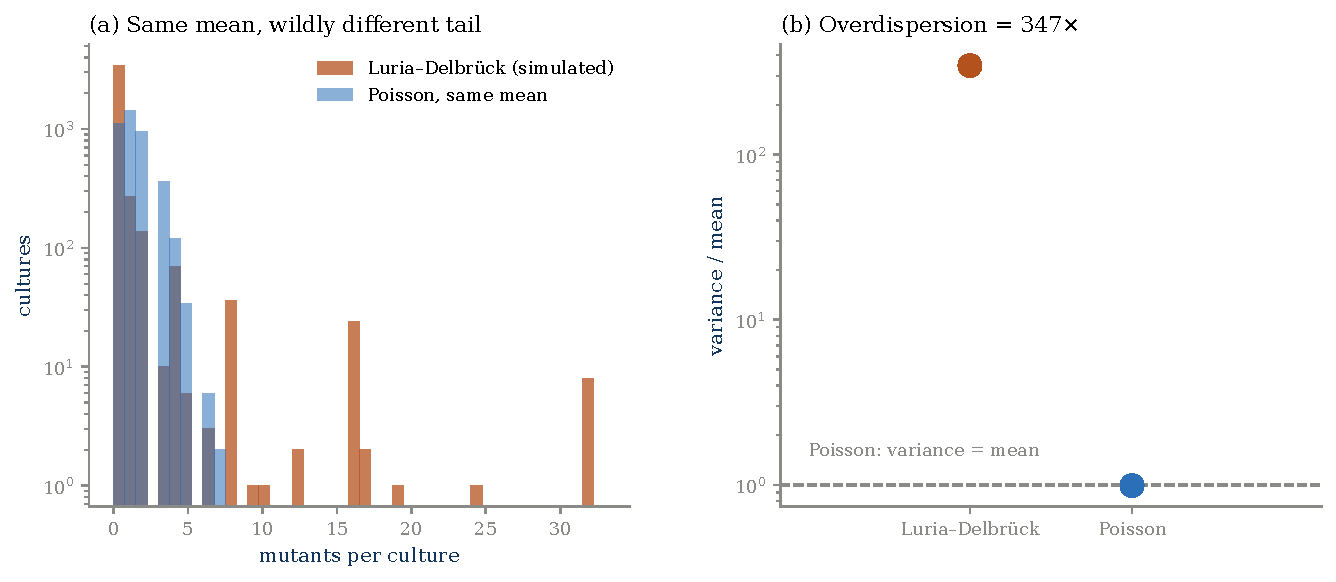
\includegraphics[width=\textwidth]{fig06_mutation_accumulation.pdf}
  \caption{(a) Simulated Luria--Delbrück counts against a Poisson distribution
  with the \emph{same mean}. The histograms are plotted on a logarithmic count
  axis; the Luria--Delbrück distribution places far more mass at zero and carries
  a tail the Poisson never reaches. (b) The variance-to-mean ratio. Each filled
  point is one reseed of the whole $4000$-culture experiment; the circled point
  is the seed quoted in the text. Every one of them falls far below the
  closed-form value (green), because $4000$ cultures cannot sample the
  first-generation events that carry the variance. The scatter, not any single
  point, is the honest summary --- see \S\ref{sub:trap}.}
  \label{fig:ld}
\end{figure}

\subsection{Consequences for Section~\ref{sec:refutation}}

Two points carry back to the refutation.

First, the rates in Table~\ref{tab:kane} are maximum-likelihood estimates from
fluctuation data, not sample means, which is why they are quoted without naive
standard errors and why their confidence intervals are asymmetric.

Second --- and this is why the ratio $\rho$ was the right statistic --- both
alleles were measured by the same protocol in the same background. Systematic
factors in the estimator (the growth model, the plating efficiency, the reporter
target size) enter both numerator and denominator and cancel. A comparison of
$\rho$ against a bound of $1$ is far more robust than either rate taken alone.

\begin{worked}[6.1: why the mode is zero]
\textbf{Problem.} With $\nu = 2\mu = 4\times10^{-8}$ and $N = 4.19\times10^{6}$,
the expected mutant count is $1.85$. Why do $85\%$ of cultures nevertheless
contain none?

\textbf{Solution.} The mean is carried by rare large clones. The total number of
wild-type divisions in a culture is $N - 1$, so the expected number of
mutational events anywhere in it is $\nu(N-1) = 0.168$, and if events are
approximately Poisson then
\[
  \Pr[\text{no event at all}] \;\approx\; e^{-0.168} \;=\; 0.845,
\]
against the simulated $0.854$. Meanwhile a single event $10$ generations from the
end contributes $2^{10} = 1024$ mutants by itself --- the observed maximum. A
distribution with most mass at zero and a mean above one must have a very heavy
tail, and that is exactly what \eqref{eq:ldvar} predicts.

Note the consistency check this provides, and what it does \emph{not} cover: the
zero-fraction is predicted to within $1\%$ because it depends only on the total
event count, a quantity $4000$ cultures sample well. The variance depends on
\emph{when} those events occur, which they sample badly. Two statistics from one
simulation, one trustworthy and one not.
\end{worked}

\begin{exercise}
Verify \eqref{eq:ldmean} by evaluating the sum directly for $g = 4$ and
$\nu = 10^{-2}$, and compare with $\tfrac{1}{2}\nu g N$.
\end{exercise}

\begin{exercise}
Show that for a Poisson random variable the variance-to-mean ratio is exactly~$1$,
and explain why any mechanism producing independent per-cell events at the moment
of challenge must give that ratio.
\end{exercise}

\begin{exercise}
The simulation uses synchronous doubling, which real cultures do not do. Argue
qualitatively whether asynchronous growth would increase or decrease the
overdispersion, and why the \emph{sign} of the Luria--Delbrück signature is robust
to this idealisation even though its magnitude is not.
\end{exercise}

\begin{exercise}[(harder)]
Suppose a variant raises $\nu$ by a factor $\rho$. Show that the \emph{ratio} of
mean mutant counts between variant and reference is $\rho$, independent of $g$
and $N$, provided both are grown identically. This is the cancellation that makes
$\rho$ in Section~\ref{sec:refutation} meaningful.
\end{exercise}

\begin{exercise}[(harder)]
Section~\ref{sub:trap} claims $4000$ cultures cannot estimate
$\operatorname{Var}[X]$. Make the claim quantitative. The variance is dominated
by events in the first few generations; require that a culture set contain, in
expectation, at least one generation-$0$ event, and deduce the number of
cultures needed at $\nu = 4\times10^{-8}$. Comment on whether the experiment is
feasible, and on what this implies for any published variance-to-mean ratio from
a fluctuation test.
\end{exercise}

\begin{ledger}
\textbf{Measured:} nothing new here; the section explains the estimator behind
the rates already quoted in Section~\ref{sec:refutation}. The simulated
quantities are computations, not measurements. \\
\textbf{Assumed:} Assumption~\ref{model:ld} --- synchronous doubling, neutral
non-reverting mutants, constant $\nu$ per cell per generation. All three are
idealisations. \\
\textbf{Proved:} nothing is formalised in this section. Equations
\eqref{eq:ldmean} and \eqref{eq:ldvar} are derived by hand. They are
\emph{not} confirmed by the simulation: \S\ref{sub:trap} shows the sample
variance falls short of \eqref{eq:ldvar} by a factor of about $550$ for a reason
the model itself explains. The mean agrees to within sampling error; the variance
is not testable at $4000$ cultures. \\
\textbf{Open:} the asynchronous-growth correction of Exercise~6.3 is not computed
anywhere in this book. Neither is the number of cultures that \emph{would} make
the variance estimable --- Exercise~6.5 asks for the order of magnitude, and it
is large enough to be a real obstacle to using this statistic at all. \\
\textbf{Corrected in this edition:} the first edition quoted the single-seed
variance-to-mean ratio of $346.7$ as the section's result, beside a closed form
predicting $190\,650$, without reconciling them or reporting that reseeding moves
the number by seventy-fold. See \S\ref{sub:trap}.
\end{ledger}
